\section{Modelo Estatico}

\begin{figure}[ht]
    \centering
    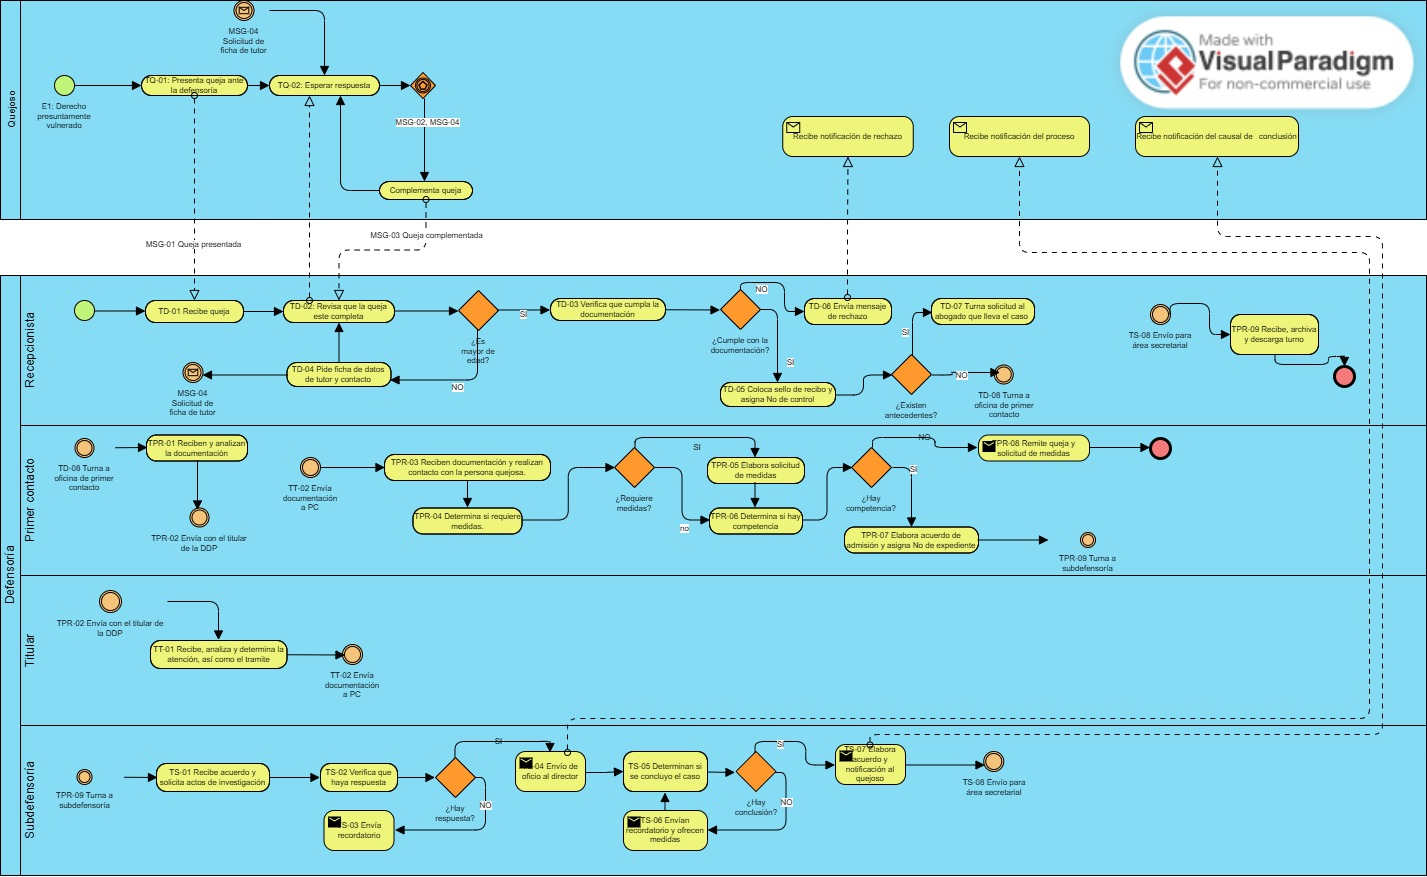
\includegraphics[width=1\textwidth]{imagenes/BMPN_Diagrama.jpg}
    \caption{Diagrama de flujo de los procesos internos de la Defensoría.}
    \label{fig:proceso_administrativo}
\end{figure}

\noindent \textbf{Descripción del flujo de trabajo:} \\

El proceso operativo inicia cuando el quejoso presenta una queja ante la defensoría por considerar vulnerados sus derechos. El caso pasa al área de Recepción, donde el personal administrativo verifica que la queja esté completa. Si el quejoso es menor de edad, se solicita la ficha de datos del tutor antes de validar la documentación técnica. Una vez confirmados los requisitos, se sella de recibido y se asigna un número de control interno. Posteriormente, se revisan antecedentes para decidir si el caso se asigna a un abogado con experiencia previa o se canaliza a Primer Contacto. Si la documentación no cumple con los requisitos, se notifica el rechazo al quejoso y se concluye el trámite. En Primer Contacto, se analiza la narrativa y las evidencias, y se puede escalar el expediente al Titular de la Defensoría para determinar la atención correspondiente. Tras contactar al quejoso, el analista evalúa la necesidad de medidas cautelares y determina la competencia del caso. Si la queja no procede, se remite a la instancia adecuada; de lo contrario, se elabora el acuerdo de admisión y se asigna un número de expediente oficial para turnarlo a la Subdefensoría. La Subdefensoría solicita y verifica los actos de investigación, gestiona las respuestas y envía recordatorios si es necesario. Una vez reunidos los elementos suficientes, se determina la conclusión del caso, se elabora el acuerdo final y se notifica al quejoso. El proceso concluye cuando el expediente se archiva en el área secretarial y se descarga el turno administrativo en el sistema de control.

